\documentclass[a4paper,utf8]{article}
\usepackage[heading,fancyhdr]{ctex}
\usepackage{amsmath,amssymb,geometry,lastpage,ulem}
\usepackage{array,tabularx,tabulary,mhchem,xspace}
\usepackage{floatrow,subfig,multirow,bigstrut}
\usepackage{siunitx,booktabs,longtable,graphicx,xfrac,nameref}
\lineskiplimit=1pt
\lineskip=3pt
\geometry{
    top=25.4mm, 
    left=25mm, 
    right=25mm, 
    bottom=25mm,
    headsep=5.9mm,
}
\ctexset{
    section = {format+=\raggedright}
}
\newcommand{\fgref}[1]{图~\ref{#1}\xspace}
\newcommand{\seqref}[1]{式~(\ref{#1})}
\newcommand{\expinfo}[7][无]{
    {\zihao{-3}\bfseries\songti
    实验名称:\uline{\hfill\mbox{#2}\hfill} \\[2.9mm]
    学\quad 号:\uline{\makebox[25mm]{#3}}\hfill
    姓\quad 名:\uline{\makebox[25mm]{#4}}\hfill
    班\quad 级:\uline{\makebox[25mm]{#5}} \\[2.9mm]
    合作者:\uline{\makebox[25mm]{#1}} \hfill
    桌\quad 号:\uline{\makebox[25mm]{#6}}\hfill\makebox[25mm+4em]{}\\[2.9mm]
    实验日期:\uline{\makebox[30mm]{#7}}\hfill\mbox{} \\[58.7mm]
    }
}
\newcommand{\pointingbox}{
    {\zihao{4}\bfseries\songti%
    实验考核\\[3mm]
    \extrarowheight=3mm
    \begin{tabularx}{150mm}{|X|X|X|X|X|}\hline
        \hfil 项目 \hfil  & \hfil 实验预习 \hfil & \hfil 实验过程 \hfil & \hfil 分析与讨论 \hfil & \hfil 总评 \hfil \\[3mm] \hline
        \hfil 评价 \hfil &  &  &  &  \\[3mm] \hline
    \end{tabularx}
    }
}
\newcommand{\derivative}[2]{\frac{\mathrm{d} #1}{\mathrm{d} #2}}
\newcommand{\thinking}[2]{\textbf{#1}\\
答:\begin{minipage}[t]{0.85\textwidth}
    #2
\end{minipage}}
\pagestyle{fancy}
\fancyhf{} \fancyhead[C]{电路基础实验} \fancyfoot[C]{\thepage~/~\pageref{LastPage}}
\newcounter{Rownumber}
\newcommand*{\Rown}{\stepcounter{Rownumber}\theRownumber}
\newcommand*{\resetRown}{\setcounter{Rownumber}{0}}
\newcommand{\qrange}[3]{\qtyrange[range-phrase = \text{$\sim$},range-units =single]{#1}{#2}{#3}}
\floatsetup[table]{capposition=top}
\newcolumntype{C}{>{\hfil}X<{\hfil}}
\renewcommand{\Nameref}[1]{\textbf{\ref{#1}~\nameref{#1}}} %导入导言
\begin{document}
\begin{center}
    {\mbox{}\\[7em]\zihao{2}\bfseries\songti%
    电路基础实验报告}\\[34mm]
    \expinfo[王慷]{元件伏安特性的测量}{22301056}{王俊杰}{22 材物}{27}{2024.5.7}
\end{center}
\newpage
\section{实验目的}
\begin{enumerate}
    \item 学习线性电阻元件和非线性电阻元件伏安特性的测试方法。
    \item 学习直流稳压电源、万用表、直流电流表、电压表的使用方法。
\end{enumerate}

\section{实验原理}%简单描述,含必要的公式和附图;
    \subsection{元件的伏安特性}
    如果把电阻元件的电压取为横坐标(纵坐标),电流取为纵坐标(横坐标),画出电压和电流的关系曲线,这条曲线称为该元件的伏安特性。
    \subsubsection{线性电阻元件}
    线性电阻元件的伏安特性在 $u-i$ 平面上是通过坐标原点的直线,与元件电压或电流的方向无关,是双向性的元件,元件上的电压和元件电流之间的关系服从欧姆定律。
        
    \subsubsection{非线性电阻元件}
    非线性电阻元件的伏安特性不是一条通过原点的直线,所以元件上电压和元件电流之间不服从欧姆定律,而元件电阻将随电压或电流的改变而改变。有些非线性电阻元件的伏安特性还与电压或电流的方向有关,也就是说,当元件两端施加的电压方向不同时,流过它的电流完全不同,如晶体二极管、发光管等,就是单向元件。
    \subsubsection{元件的伏安特性}
    可以通过实验方法测定。用电流表、电压表测定伏安特性的方法,叫伏安法。测试线性电阻元件的伏安特性,可采用改变元件两端电压测电流的方法得到,或采取改变通过元件的电流而测电压的方法得到。
\section{实验仪表}
    RIGOL DM3058 万用表、RIGOL DP832 直流稳压电源、电路分析实验箱、导线若干。
\section{实验内容及实验数据}
    \subsection{测试线性电阻元件的伏安特性}
    用电压表和电流表分别采用方法一(电流表外接法)和方法二(电流表内接法)的两种接线方法进行测试,比较测试结果。一下简称外接法和内接法。
    \begin{enumerate}
        \item 线性电阻元件的正向特性测量,分别采用方法一和方法二。
        \item 反向特性测量,改变加在电阻元件两端电压的方向,测量时应注意电压表,电流表正负极接入的方向。
        \item 计算电阻值,是根据测量的电压、电流值进行计算。
    \end{enumerate}
    \begin{table}[!ht]
        \centering
        \subfloat[给定电压]{\begin{tabular}{S[table-format=2.0] *{2}{S[table-format=2.2]}} \toprule
            {\parbox{2.1em}{\centering 电压\\(\unit{\V})}} & {\parbox{5.1em}{\centering 外接法电流\\(\unit{\mA})}} & {\parbox{5.1em}{\centering 内接法电流\\(\unit{\mA})}}  \\[7pt] \midrule
            10 & 83.23 & 83.87  \\ 
            8 & 68.12 & 67.35  \\ 
            6 & 50.95 & 50.46  \\ 
            4 & 33.87 & 33.59  \\ 
            2 & 16.84 & 16.76  \\ 
            0 & 0 & 0  \\ 
            -2 & -16.83 & -16.72  \\ 
            -4 & -33.88 & -33.45  \\ 
            -6 & -51.01 & -50.19  \\ 
            -8 & -68.45 & -67.03  \\ 
            -10 & -85.64 & -84.16  \\ \bottomrule
        \end{tabular}}\hfil
        \subfloat[给定电流]{\begin{tabular}{S[table-format=2.0] *{2}{S[table-format=2.2]}} \toprule
            {\parbox{2.1em}{\centering 电流\\(\unit{\mA})}} & {\parbox{5.1em}{\centering 外接法电压\\(\unit{\V})}} & {\parbox{5.1em}{\centering 内接法电压\\(\unit{\V})}}  \\[7pt] \midrule
            10 & 1.182 & 1.204  \\ 
            8 & 0.947 & 0.963  \\ 
            6 & 0.710 & 0.723  \\ 
            4 & 0.473 & 0.481  \\ 
            2 & 0.237 & 0.241  \\ 
            0 & 0 & 0  \\ 
            -2 & -0.237 & -0.242  \\ 
            -4 & -0.474 & -0.483  \\ 
            -6 & -0.711 & -0.723  \\ 
            -8 & -0.948 & -0.964  \\ 
            -10 & -1.185 & -1.205  \\ \bottomrule
        \end{tabular}}
        \caption{线性电阻元件的伏安特性测量结果}
    \end{table}

    \subsection{测试非线性电阻元件 D3(二极管)、D4(发光二极管)的伏安特性}
    \begin{enumerate}
        \item 正向特性的测试。为使特性曲线测得准确,先从低到高给出一定电压(电流)值(不能超过规定值),预测一次,由预测结果描出曲线的草图,然后再根据曲线形状合理选取电压(电流)值进行正式测量。曲线曲率大的地方,测量点要选密些,反之疏些,一定要测出拐点、导通电压(电流突然变大)等有特征的点,达到能完整、真实的测出元件的特性曲线。
        \item 反向特性的测试。
    \end{enumerate}
    \begin{table}[!ht]
        \centering
        \subfloat[外接法]{\begin{tabular}{*{4}{S[table-format=2.3]}} \toprule
            {\parbox{4.1em}{\centering 正向电压\\(\unit{\V})}} & {\parbox{4.1em}{\centering 正向电流\\(\unit{\mA})}} & {\parbox{4.1em}{\centering 反向电压\\(\unit{\V})}} & {\parbox{4.1em}{\centering 反向电流\\(\unit{\uA})}} \\ \midrule
            0.000 & 0.000 & 0.000 & 0.000 \\
            0.396 & 0.027 & 2.000 & 0.203 \\
            0.456 & 0.124 & 4.000 & 0.405 \\
            0.486 & 0.249 & 6.000 & 0.604 \\
            0.517 & 0.502 & 8.000 & 0.805 \\
            0.549 & 1.000 & 10.000 & 1.006 \\
            0.581 & 2.000 & 12.000 & 1.206 \\
            0.601 & 3.010 & 14.000 & 1.406 \\
            0.624 & 4.994 & 16.000 & 1.607 \\
            0.643 & 7.550 & 18.000 & 1.808 \\
            0.655 & 10.040 & 20.000 & 2.007 \\ \bottomrule
        \end{tabular}}\hfil
        \subfloat[内接法]{\begin{tabular}{*{4}{S[table-format=2.3]}} \toprule
            {\parbox{4.1em}{\centering 正向电压\\(\unit{\V})}} & {\parbox{4.1em}{\centering 正向电流\\(\unit{\mA})}} & {\parbox{4.1em}{\centering 反向电压\\(\unit{\V})}} & {\parbox{4.1em}{\centering 反向电流\\(\unit{\uA})}} \\ \midrule
            0.000 & 0.000 & 0.000 & 0.000 \\
            0.391 & 0.023 & 2.000 & 0.002 \\
            0.471 & 0.172 & 4.000 & 0.003 \\
            0.500 & 0.336 & 6.000 & 0.003 \\
            0.530 & 0.639 & 8.000 & 0.004 \\
            0.552 & 1.010 & 10.000 & 0.005 \\
            0.578 & 1.720 & 12.000 & 0.006 \\
            0.605 & 3.000 & 14.000 & 0.006 \\
            0.632 & 4.960 & 16.000 & 0.006 \\
            0.654 & 7.440 & 18.000 & 0.007 \\
            0.671 & 9.950 & 20.000 & 0.008 \\ \bottomrule
        \end{tabular}}
        \caption{D3 的伏安特性测量结果}
    \end{table}
    \begin{table}[!ht]
        \centering
        \subfloat[外接法]{\begin{tabular}{*{4}{S[table-format=2.3]}} \toprule
            {\parbox{4.1em}{\centering 正向电压\\(\unit{\V})}} & {\parbox{4.1em}{\centering 正向电流\\(\unit{\mA})}} & {\parbox{4.1em}{\centering 反向电压\\(\unit{\V})}} & {\parbox{4.1em}{\centering 反向电流\\(\unit{\uA})}} \\ \midrule
            0.000  & 0.000  & 0.000  & 0.000   \\ 
            1.570  & 0.001  & 2.000  & 0.199   \\ 
            1.696  & 0.010  & 4.000  & 0.399   \\ 
            1.799  & 0.050  & 6.000  & 0.600   \\ 
            1.998  & 0.200  & 8.000  & 0.800   \\ 
            2.331  & 0.500  & 10.000  & 1.001   \\ 
            2.858  & 1.000  & 12.000  & 1.202   \\ 
            3.887  & 2.000  & 14.000  & 1.402   \\ 
            5.919  & 4.000  & 16.000  & 1.603   \\ 
            7.936  & 6.000  & 18.000  & 1.804   \\ 
            11.950  & 10.000  & 20.000  & 2.005   \\ \bottomrule
        \end{tabular}}\hfil
        \subfloat[内接法]{\begin{tabular}{*{4}{S[table-format=2.3]}} \toprule
            {\parbox{4.1em}{\centering 正向电压\\(\unit{\V})}} & {\parbox{4.1em}{\centering 正向电流\\(\unit{\mA})}} & {\parbox{4.1em}{\centering 反向电压\\(\unit{\V})}} & {\parbox{4.1em}{\centering 反向电流\\(\unit{\uA})}} \\ \midrule
            0.000  & 0.000  & 0.000  & 0.000   \\ 
            1.799  & 0.050  & 10.000  & 0.000   \\ 
            1.874  & 0.100  & 12.000  & 0.001   \\ 
            1.998  & 0.200  & 13.000  & 0.001   \\ 
            2.223  & 0.400  & 14.000  & 0.001   \\ 
            2.438  & 0.600  & 15.000  & 0.002   \\ 
            2.858  & 1.000  & 16.000  & 0.002   \\ 
            3.889  & 2.000  & 17.000  & 0.003   \\ 
            5.924  & 4.000  & 18.000  & 0.004   \\ 
            7.940  & 6.000  & 19.000  & 0.004   \\ 
            11.970  & 10.000  & 20.000  & 0.005   \\ \bottomrule
        \end{tabular}}
        \caption{D4 的伏安特性测量结果}
    \end{table}

\section{实验结果与分析}
对线性电阻元件测得的伏安特性曲线拟合,可以得到其电阻
\begin{table}[!ht]
    \caption{线性电阻元件电阻值测量值}
    \begin{tabular}{ccccc} \toprule
         & 给定电压外接 & 给定电压内接 & 给定电流外接 & 给定电流内接 \\ \midrule
        测量值(\unit{\ohm}) & 117.92 & 119.10 & 118.39 & 120.46 \\ \bottomrule
    \end{tabular}
\end{table}
将上述实验数据绘图可得\par
\begin{figure}[!ht]
    \caption{D3 伏安特性曲线}
    \subfloat[D3 外接法]{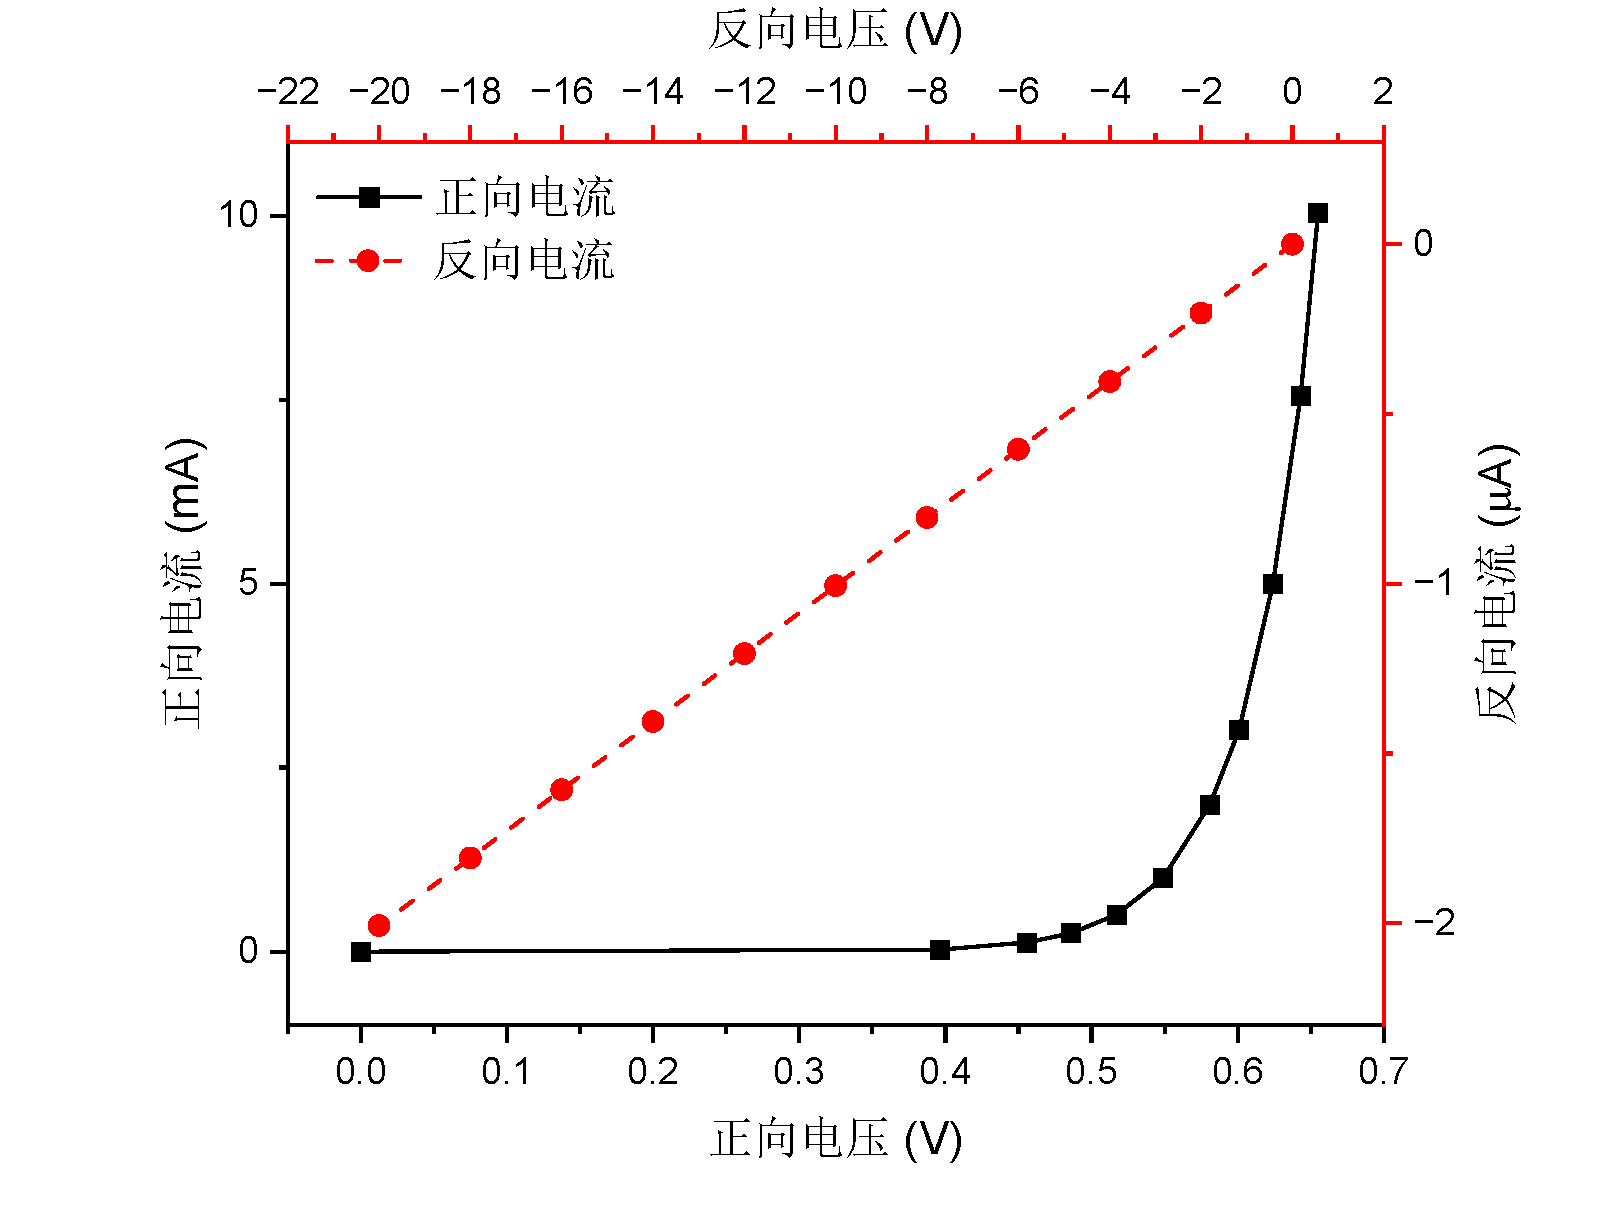
\includegraphics[width=0.45\textwidth]{D3out.pdf}}
    \subfloat[D3 内接法]{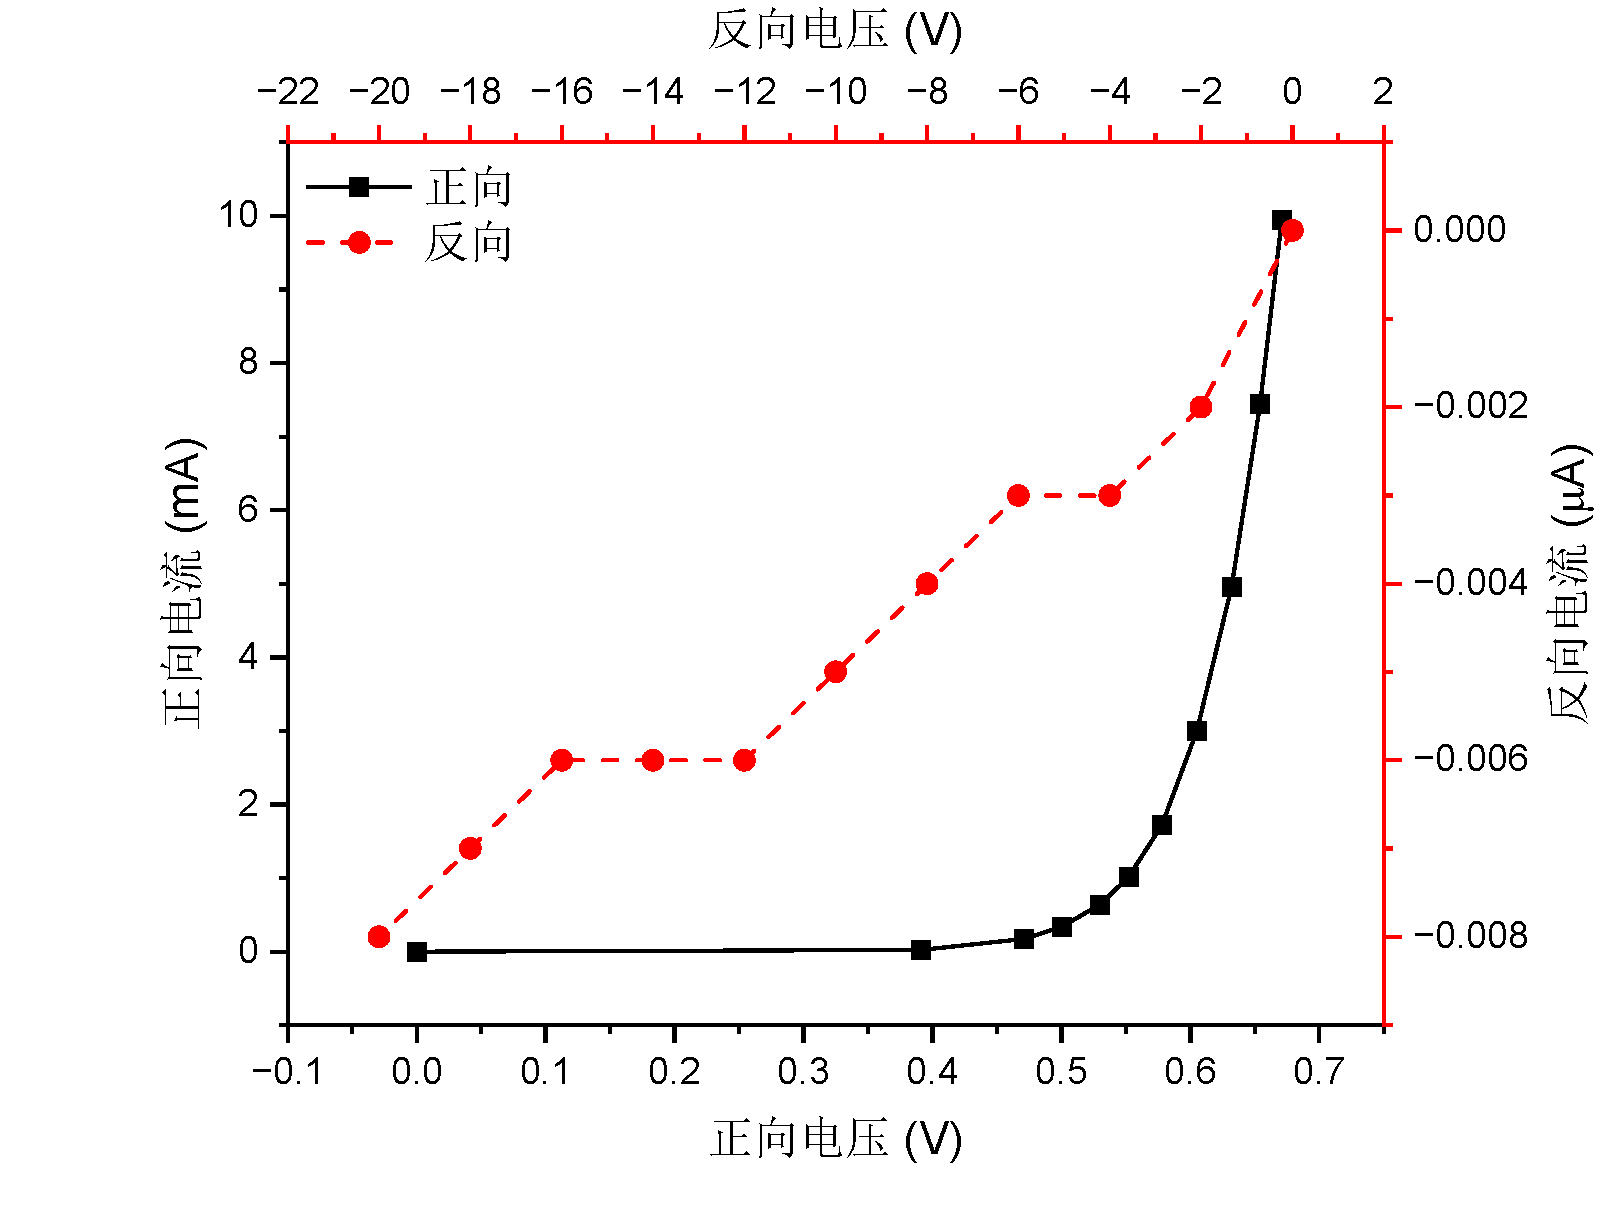
\includegraphics[width=0.45\textwidth]{D3in.pdf}}
\end{figure}
\begin{figure}[!ht]
    \caption{D3 伏安特性曲线}
    \subfloat[D4 外接法]{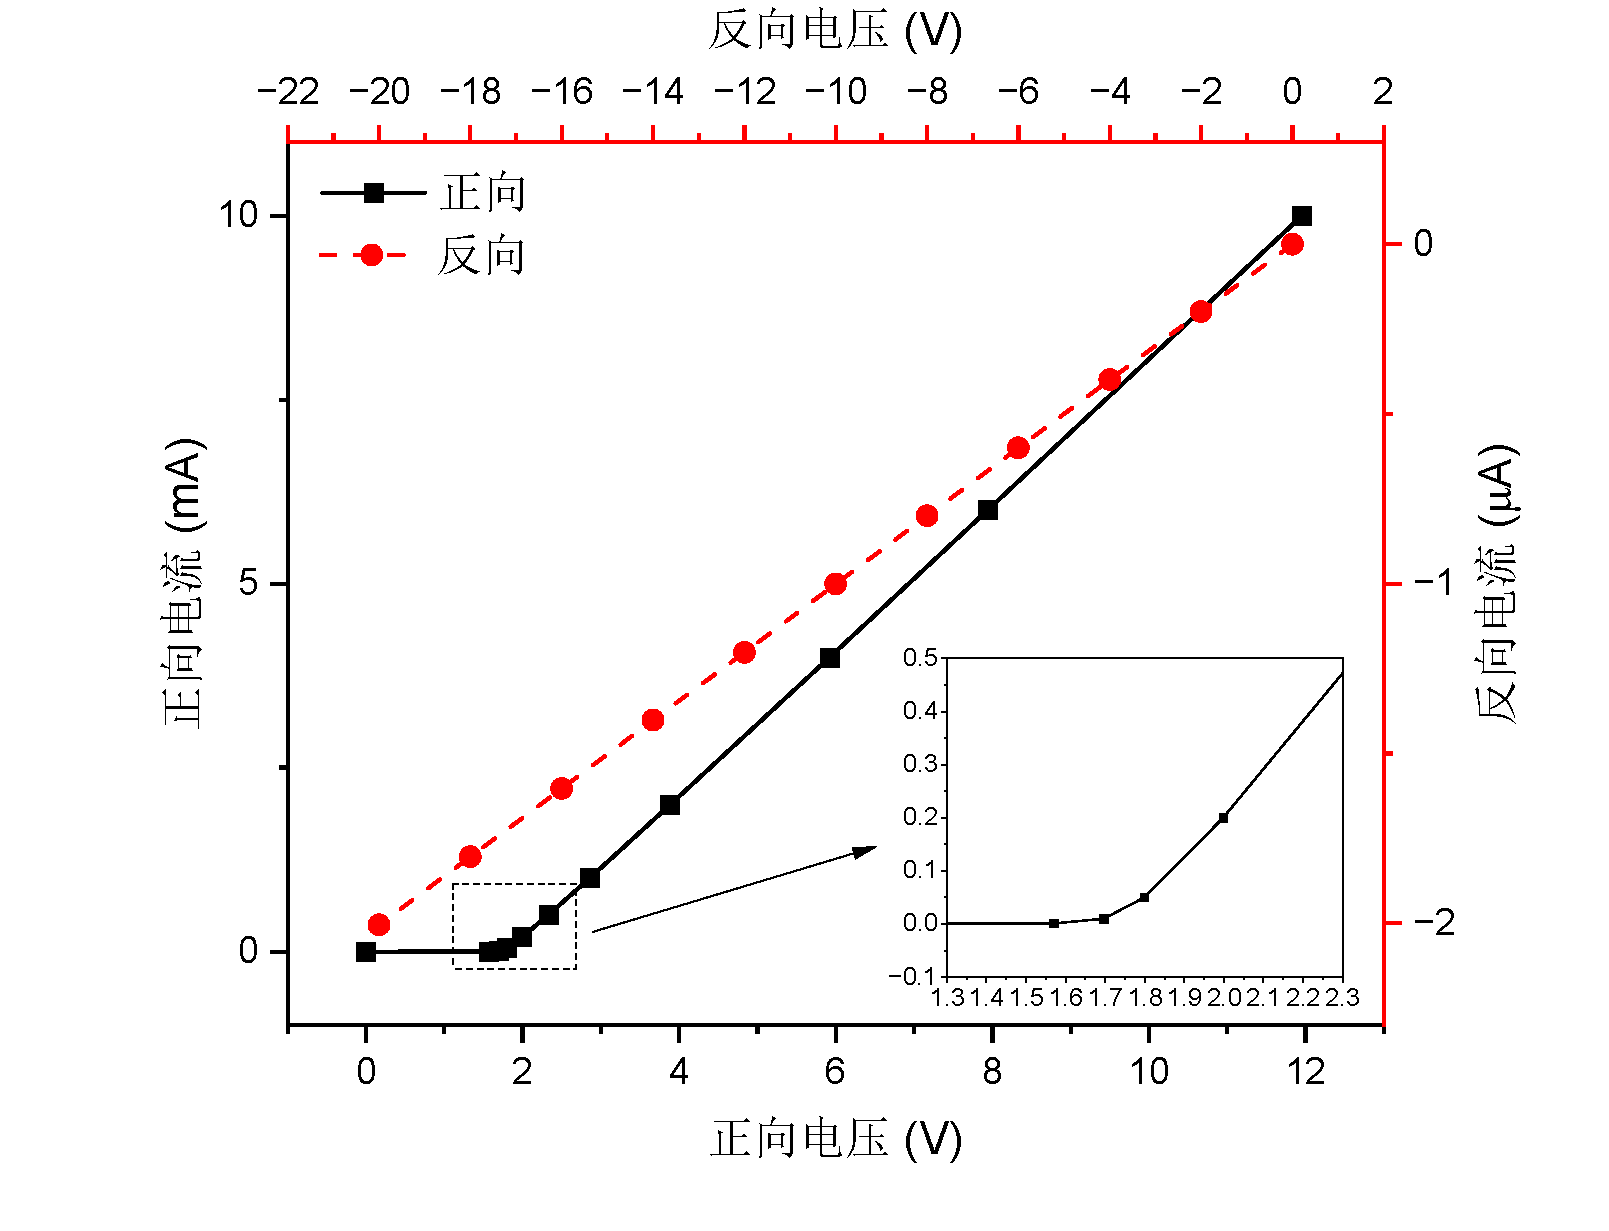
\includegraphics[width=0.45\textwidth]{D4out.pdf}}
    \subfloat[D4 内接法]{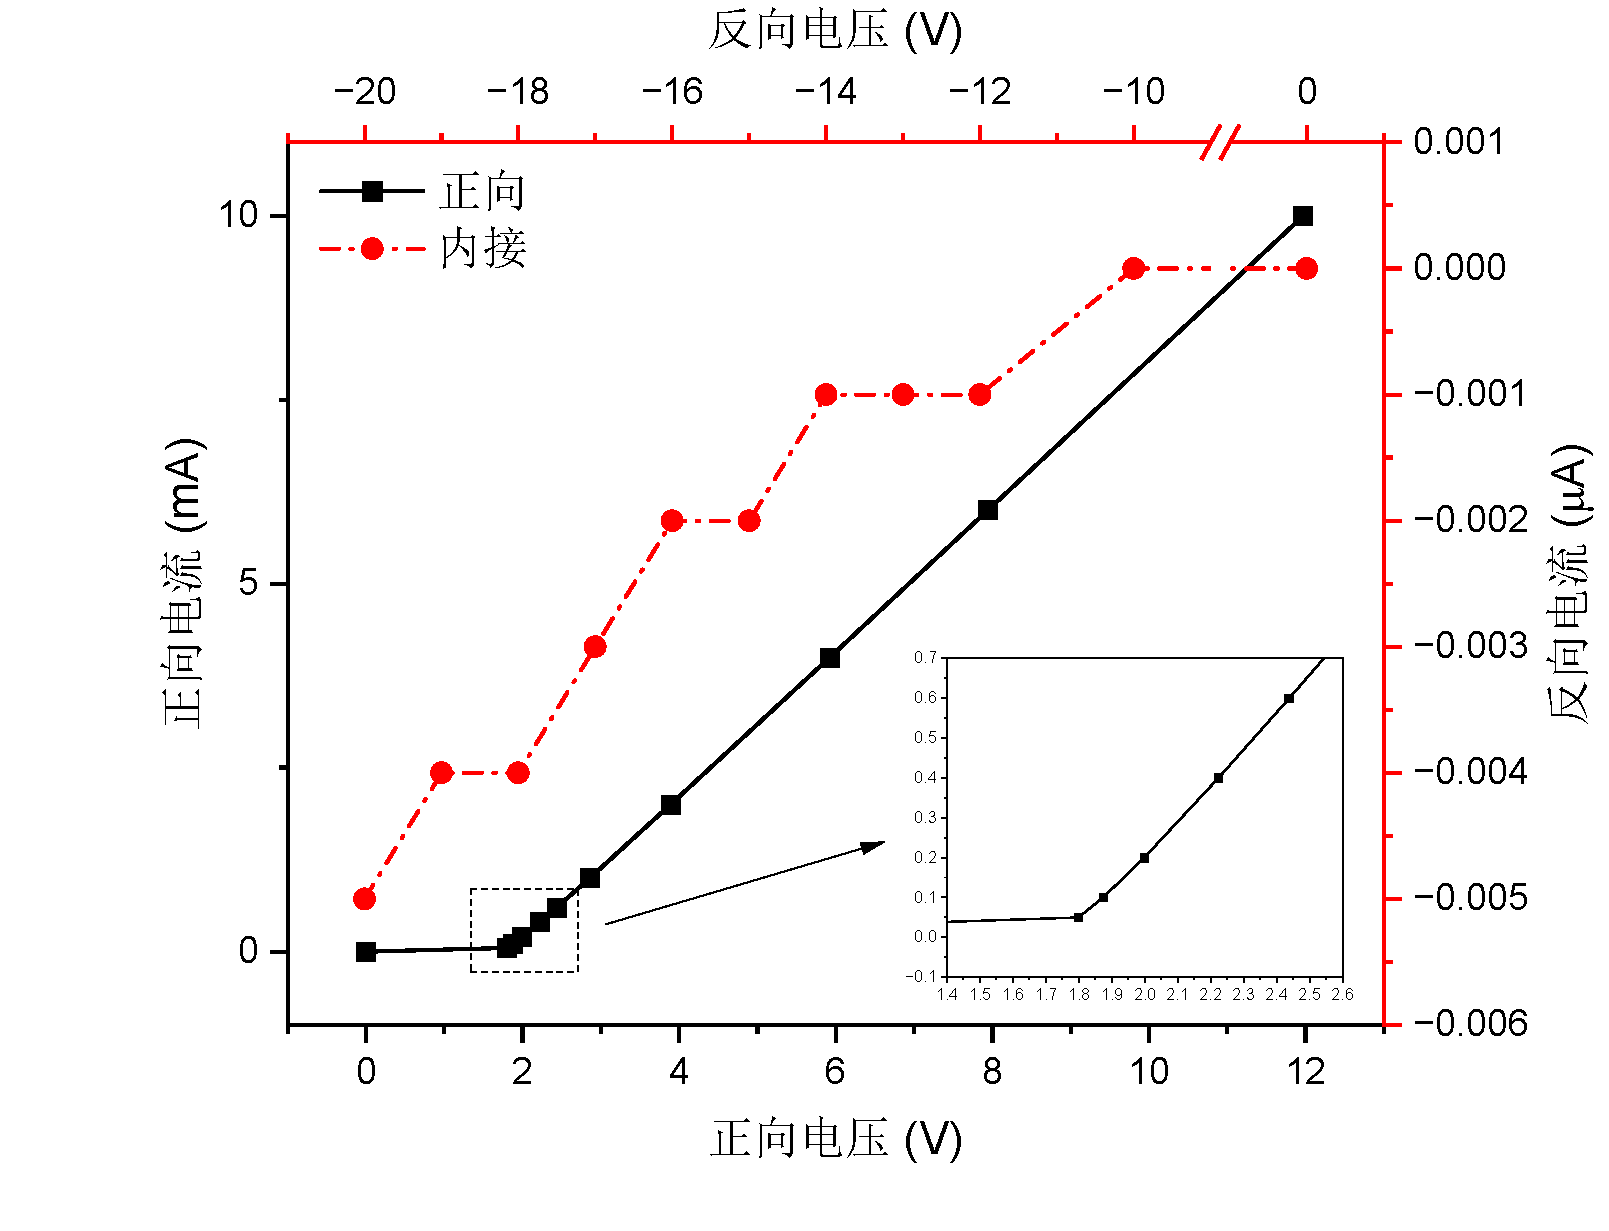
\includegraphics[width=0.45\textwidth]{D4in.pdf}}
\end{figure}
\begin{figure}[!ht]
    \caption{线性电阻元件伏安特性曲线}
    \subfloat[外接法 $u-i$]{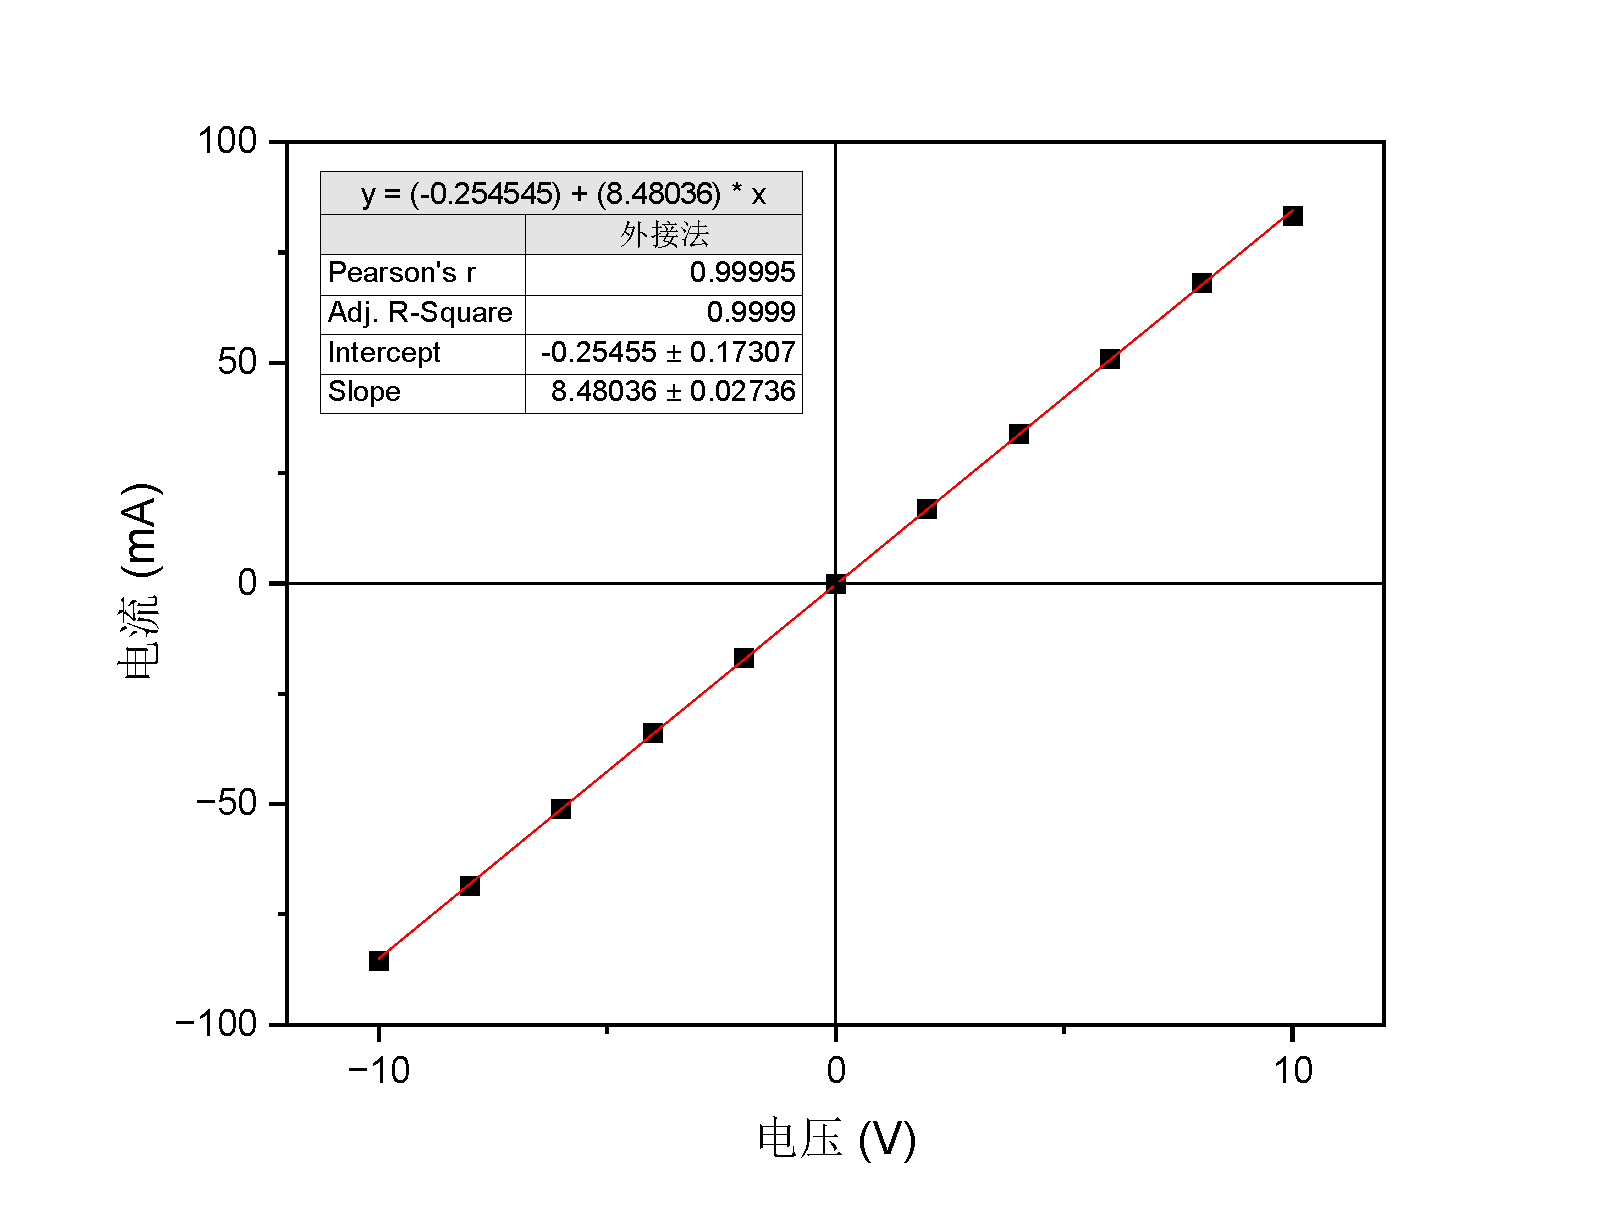
\includegraphics[width=0.45\textwidth]{1Vout.pdf}}
    \subfloat[内接法 $u-i$]{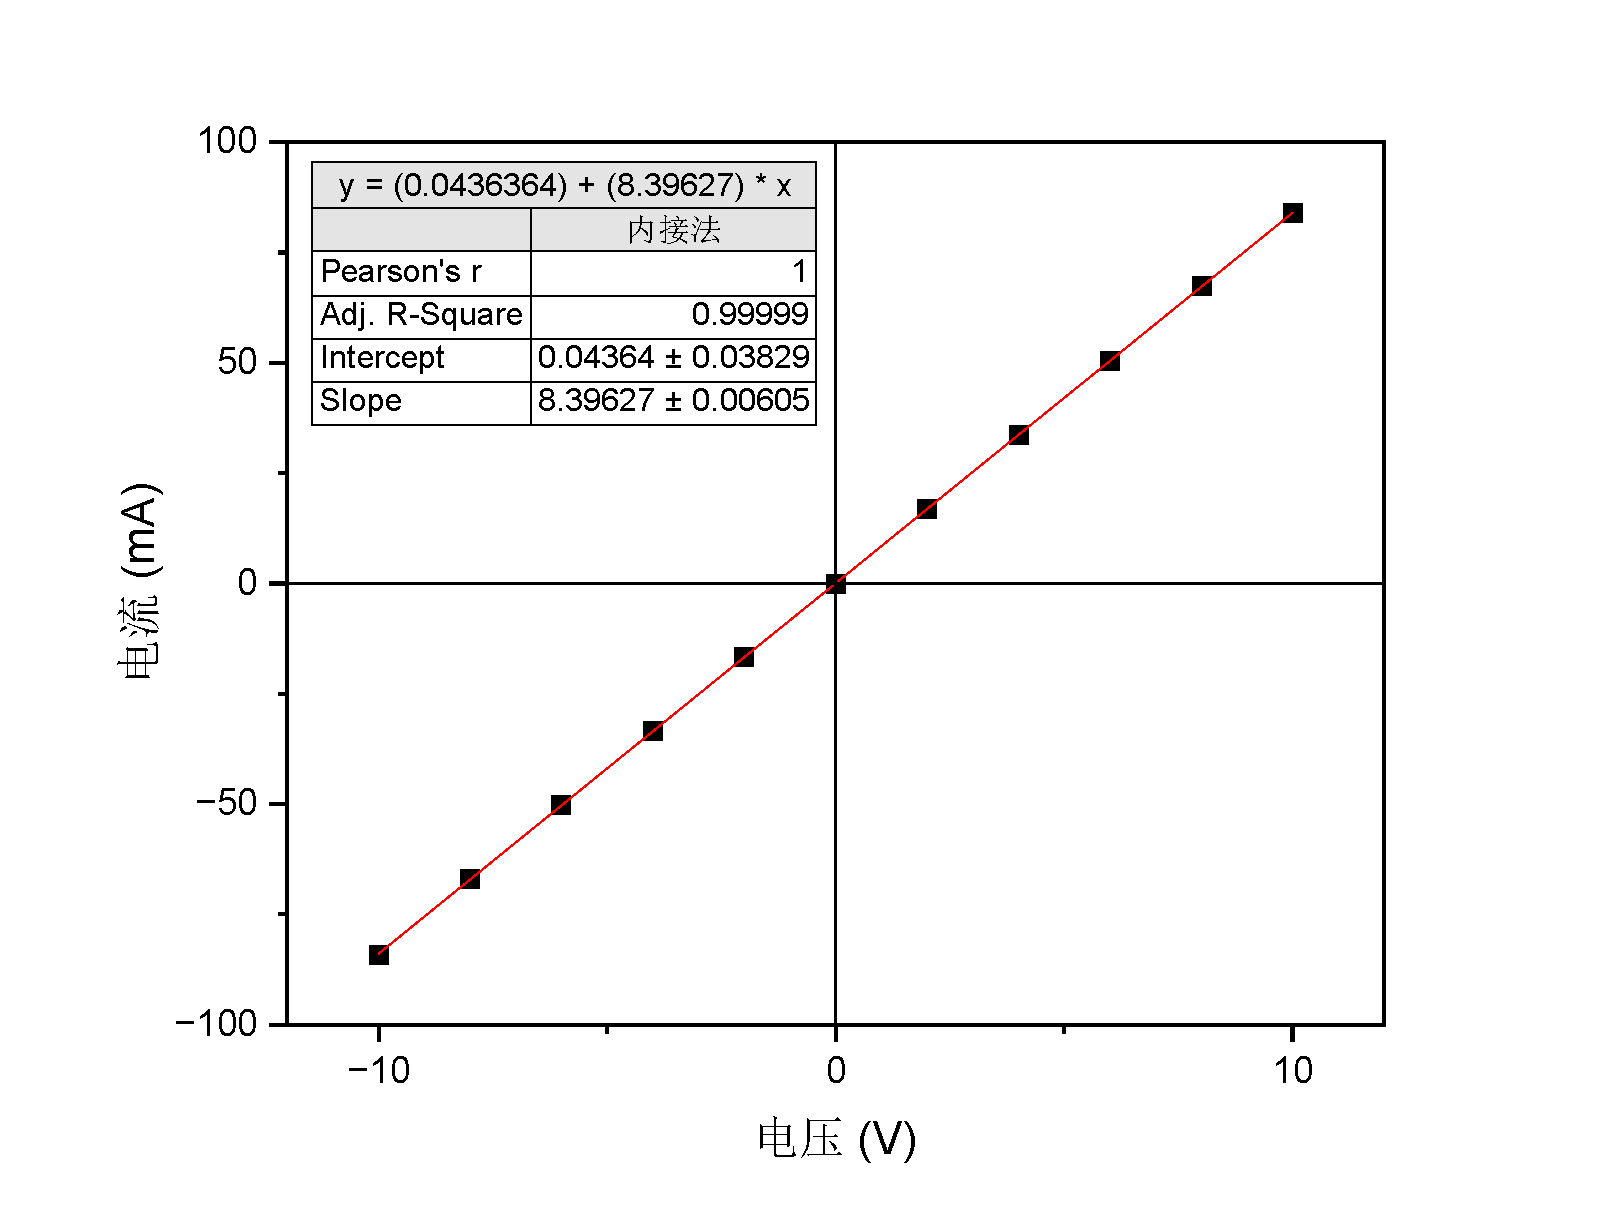
\includegraphics[width=0.45\textwidth]{1Vin.pdf}}\\
    \subfloat[外接法 $i-u$]{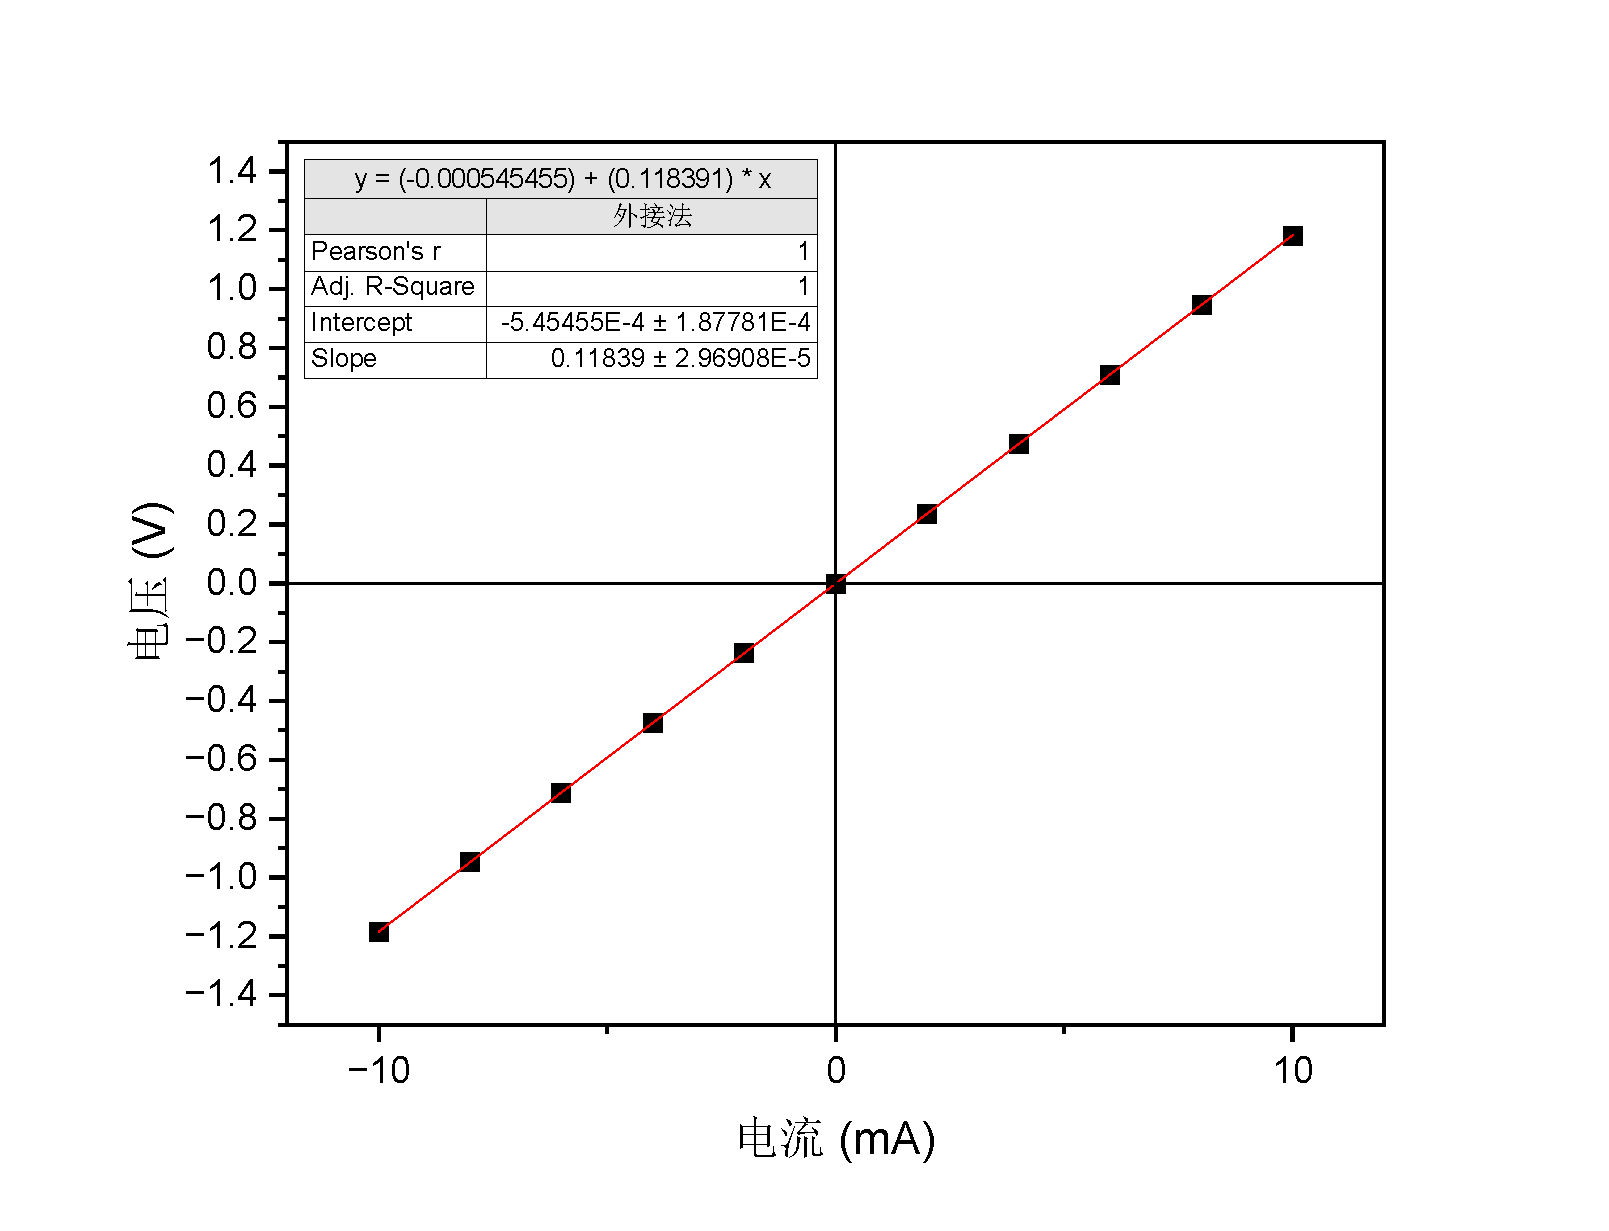
\includegraphics[width=0.45\textwidth]{1Iout.pdf}}
    \subfloat[内接法 $i-u$]{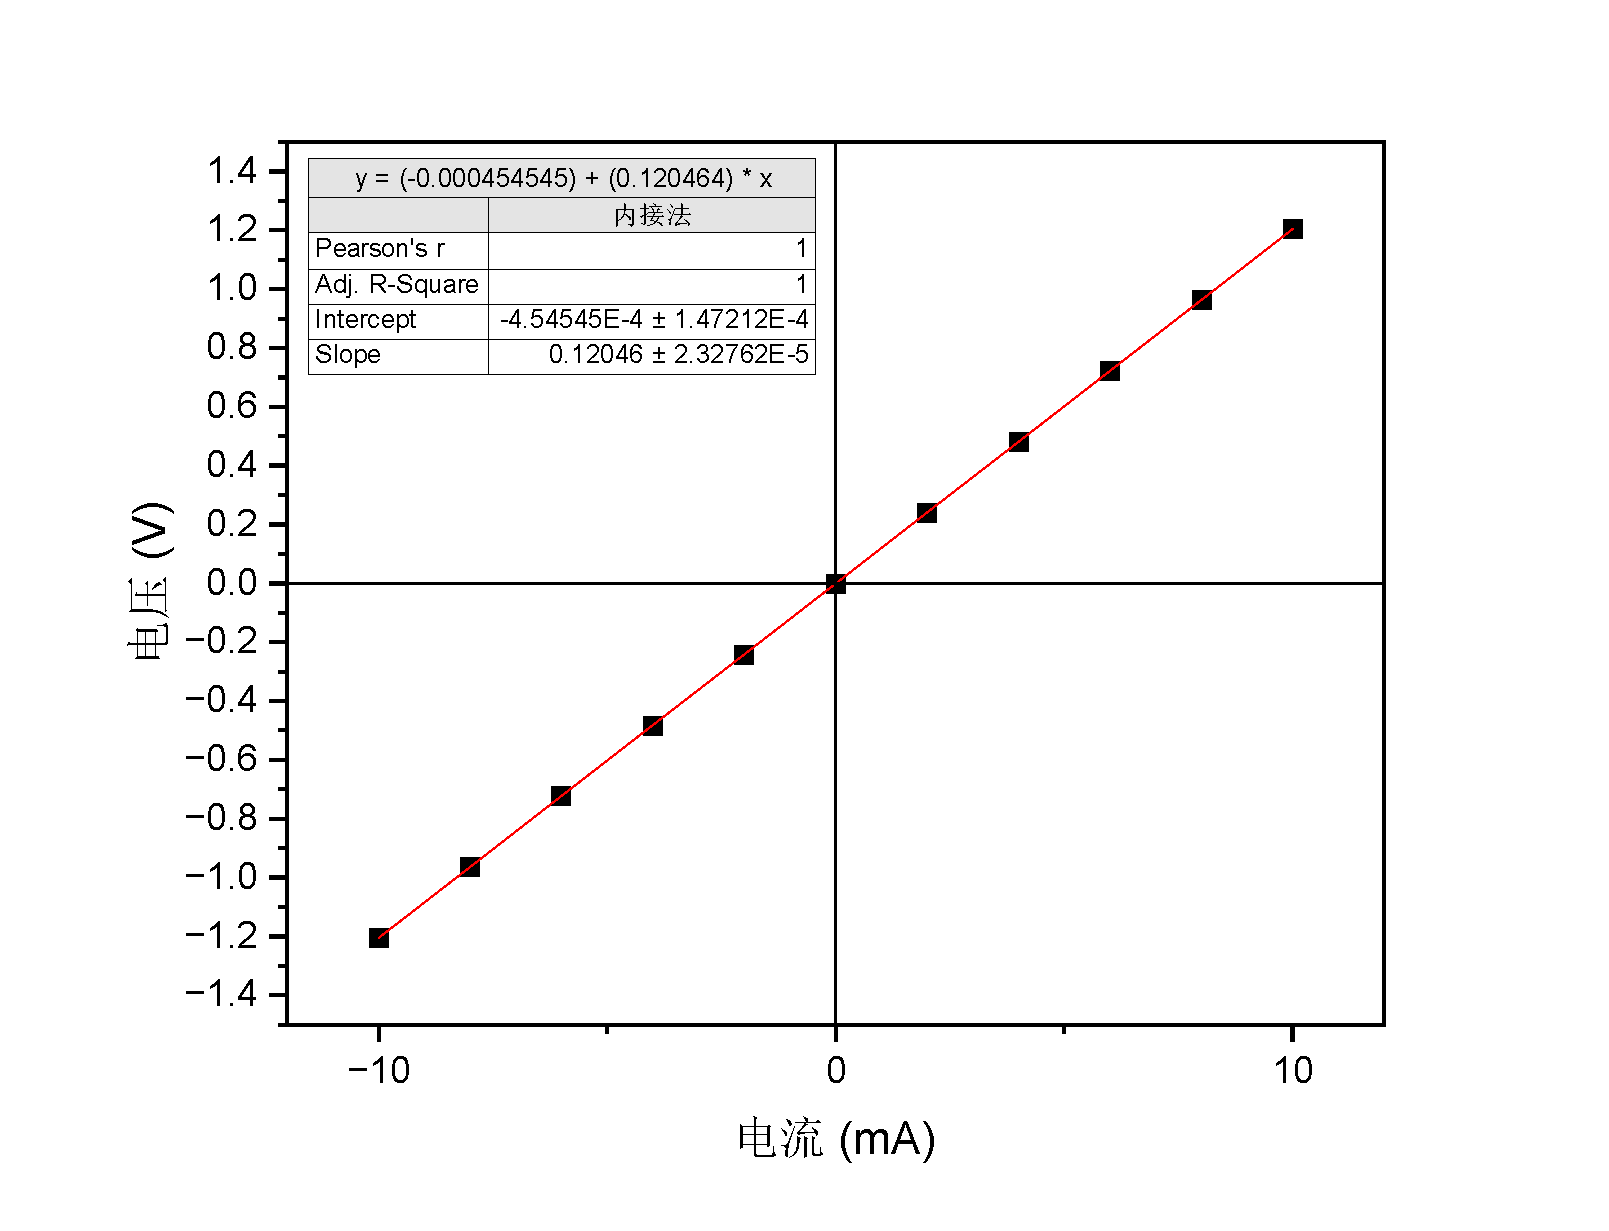
\includegraphics[width=0.45\textwidth]{1Iin.pdf}}\\
\end{figure}
\clearpage
\subsection{数据分析}
根据内接法和外接法的电路图分析可得
\begin{align*}
    \text{电压表外接法:}&R_\text{测}=R_\text{A}+R_\text{真} > R_\text{真} \\
    \text{电流表外接法:}&R_\text{测}=\frac{R_\text{V} R_\text{真}}{R_\text{V}+R_\text{真}} < R_\text{真}
\end{align*}
考虑到电流小时仪器相对误差偏大,故可以认为该 \SI{120}{\ohm} 的电阻实际阻值应该在 \SI{117.92}{\ohm} 到 \SI{119.10}{\ohm} 之间。而两个二极管有很明显的单向性,反向加压时电阻极大,甚至比电压表的电阻大很多。但正向导通后电阻很小且几乎为线性。
\subsection{误差分析}
此次实验的误差来源有:
\begin{enumerate}
    \item 测试线路上的电阻、寄生电容
    \item 测量时的接触不良也可能产生误差
    \item 实验原理本身的系统误差
    \item 实验当天温度、湿度的影响
    \item 人为读数时引入的误差
\end{enumerate}
\section{思考题}
\subsection{线性电阻元件的两个特殊情况“开路”、“短路”的含义是什么?}
\begin{enumerate}
    \item 开路
    \begin{itemize}
        \item \textbf{含义}:开路指的是电路中有一段断开,没有电流通过。
        \item \textbf{特性}:在这种情况下,电阻是无限大的,电流为零。电压可以存在,但由于没有电流流动,电路中不会有能量传递。
    \end{itemize}
    \item 短路
    \begin{itemize}
        \item \textbf{含义}:短路指的是电路中某段电阻接近于零,导致电流非常大。
        \item \textbf{特性}:在这种情况下,电阻非常小,几乎为零,电流会非常大。由于过大的电流,可能会导致电路过热,甚至损坏电路中的元件。
    \end{itemize}
\end{enumerate}
\subsection{试说明可调三端电阻最常见的三个用途}
\begin{enumerate}
    \item 电压分压器
    \begin{itemize}
        \item \textbf{用途}:通过调整电位器的滑动端的位置,可以在其两端之间得到一个可调的输出电压。这种方法广泛用于调节输入信号电压、设置参考电压等。
        \item \textbf{描述}:在电位器上,$V_{\text{in}}$ 施加在固定端,$V_{\text{out}}$ 从滑动端取出。通过改变滑动端的位置,可以调节 $R_1$ 和 $R_2$ 的比例,从而调节输出电压。
    \end{itemize}
    \item 调节电流
    \begin{itemize}
        \item \textbf{用途}:可变电阻器可用来控制电路中的电流。例如,在 LED 电路中,通过调整电阻值,可以控制通过 LED 的电流,从而改变其亮度。
        \item \textbf{描述}:在一个简单的电路中,电源电压 $V$ 固定,通过调整电位器的阻值 $R$,可以改变流经电路的电流 $I$。
    \end{itemize}
    \item 信号调节
    \begin{itemize}
        \item \textbf{用途}:在音频设备中,电位器常用于调节音量、电平、音调等参数。通过旋转电位器的旋钮,可以方便地调节输出信号的强度或特性。
        \item \textbf{描述}:电位器作为信号调节器,通过改变其位置,可以调整输入信号的增益 $k$,从而改变输出信号的幅度。
    \end{itemize}
\end{enumerate}
\subsection{思考题 3}
电流表应与被测元件\uline{\makebox[3em]{串}}联,电压表应与被测元件\uline{\makebox[3em]{并}}联,电流表、电压表都有内阻,而电流表内阻应越\uline{\makebox[3em]{小}}越好,电压表内阻应越\uline{\makebox[3em]{大}}越好,这是因为:
\begin{itemize}
    \item 电流表的内阻越小,它对电路的影响就越小。若电流表有较大的内阻,会在电流表上产生电压降,改变电路中原有的电流分布,导致测量误差。理想情况下,电流表的内阻为零,不改变电路中的电流。
    \item 电压表的内阻越大,它对电路的影响就越小。若电压表有较小的内阻,会引起分流,改变被测元件两端的电压,导致测量误差。理想情况下,电压表的内阻为无穷大,不改变被测元件两端的电压。
\end{itemize}
\subsection{试分析接入电路的电流表内阻大、电压表内阻小时,对测试结果有何影响?}
\subsubsection{电流表内阻大}
\begin{itemize}
    \item \textbf{影响}:电流表的内阻大意味着电流表本身在电路中引入了一个额外的电阻。这会导致几个问题:
    \begin{itemize}
        \item \textbf{电流减小}:由于电流表内阻的存在,整个电路的总电阻增大,导致通过电路的电流减小。这样,电流表测得的电流值会比实际电流值小。
        \item \textbf{测量误差}:增加的内阻会导致电流表上的电压降,从而改变电路中其他元件的电压分布,导致测量误差。
    \end{itemize}
    \item \textbf{示例}:
    若电路中有一个电阻 $R$ 和电源电压 $V$,电流表内阻为 $R_m$。电流表测得的电流为:
    \begin{equation}
    I = \frac{V}{R + R_m}
    \end{equation}
    由于 $R_m$ 增大, $I$ 将减小,与真实电流 $\frac{V}{R}$ 相比,产生误差。
\end{itemize}

\subsubsection{电压表内阻小}
\begin{itemize}
    \item \textbf{影响}:电压表的内阻小意味着电压表在测量时会引入额外的电流,导致以下问题:
    \begin{itemize}
        \item \textbf{电压减小}:电压表内阻小,会引起显著的分流作用,使被测元件两端的电压下降。这样,电压表测得的电压值会比实际电压值小。
        \item \textbf{测量误差}:电压表内阻小会改变电路的电流分布,特别是高阻抗电路中,这种影响更为显著。
    \end{itemize}
    \item \textbf{示例}:
    若电压表内阻为 $R_v$,被测电阻为 $R$,施加的电压为 $V$,并联后的总电阻为:
    \begin{equation}
    R_{\text{total}} = \frac{R R_v}{R + R_v}
    \end{equation}
    电压表测得的电压为:
    \begin{equation}
    V_{\text{out}} = I \cdot R_{\text{total}} = V \cdot \frac{R_{\text{total}}}{R + R_{\text{total}}}
    \end{equation}
    若 $R_v$ 很小,则 $R_{\text{total}} \approx R_v$,导致 $V_{\text{out}}$ 显著小于 $V$,从而产生误差。
\end{itemize}
\subsection{如果被测元件阻值小应采用电流表外接法不是电压表外接法?被测元件阻值大又应如何连接?为什么?}
\subsubsection{被测元件阻值小:采用电流表外接法}
\begin{itemize}
    \item \textbf{连接方式}:将电流表与被测元件串联,并在电流表外部接入电压表。
    \item \textbf{理由}:
    \begin{itemize}
        \item 当被测元件的阻值很小时,电流表内阻($R_\text{A}$)相对于被测元件的阻值可能不容忽视。如果采用电流表内接法,电流表内阻会显著影响测量精度。
        \item 电流表外接法将电流表内阻的影响降到最低,因为电压表并联在电流表和被测元件的组合上。这样,测量电压时不会受电流表内阻的影响。
        \item 在这种连接方式中,电流表直接测量通过被测元件的电流,电压表测量整个回路的电压。
    \end{itemize}
\end{itemize}

\subsubsection{被测元件阻值大:采用电压表外接法}

\begin{itemize}
    \item \textbf{连接方式}:将电压表与被测元件并联,并在电压表外部接入电流表。
    \item \textbf{理由}:
    \begin{itemize}
        \item 当被测元件的阻值很大时,电压表内阻($R_\text{V}$)相对于被测元件的阻值可能不容忽视。如果采用电压表内接法,电压表内阻会显著影响测量精度。
        \item 电压表外接法将电压表内阻的影响降到最低,因为电流表串联在整个回路中,电压表直接测量被测元件的电压。
        \item 在这种连接方式中,电流表测量总电流,电压表测量被测元件的电压。
    \end{itemize}
\end{itemize}

\section{实验心得}
此次实验测量了大量数据,但经过数据处理后,绘制的图像效果不错。实验采取了不同方法来测量同一元件的伏安特性,让我们感受到各个方法间的不同之处。就比如二极管的反向特性测量应该使用电压表外接的方法测量。
\section{原始数据}
    \begin{figure}[!ht]
        \framebox{\includegraphics*[width=0.94\textwidth]{data.jpg}}
    \end{figure}
\end{document}